\subsection{Model Selection} \label{meth-encode-model-subsect}
To perform model selection we used the Bayesian Information Criterion \citep{Schwarz1978}. \emph{Fig. \ref{model-BIC-pic}} shows how BIC score changes as we increase the number of clusters K for (a) K562 cell line and (b) H1-hESC cell line. In both plots as we increase K, BIC score also increases; however, around K=5 we find a plateau where the BIC score does not change significantly as we increase the complexity of the model. Someone would expect the BIC score to gradually increase, and after reaching a peak value to start decreasing, since the model would be penalized more for its added complexity. This is not the case in our experiments because of the large values of the log-likelihood. Even though BIC penalizes heavily more complex models, its penalty is not so strong enough to overcome the increase of log-likelihood as the model fits better the data. 
\begin{figure}[ht!]
     \begin{center}
        \subfigure[]{
            \label{model:first}
            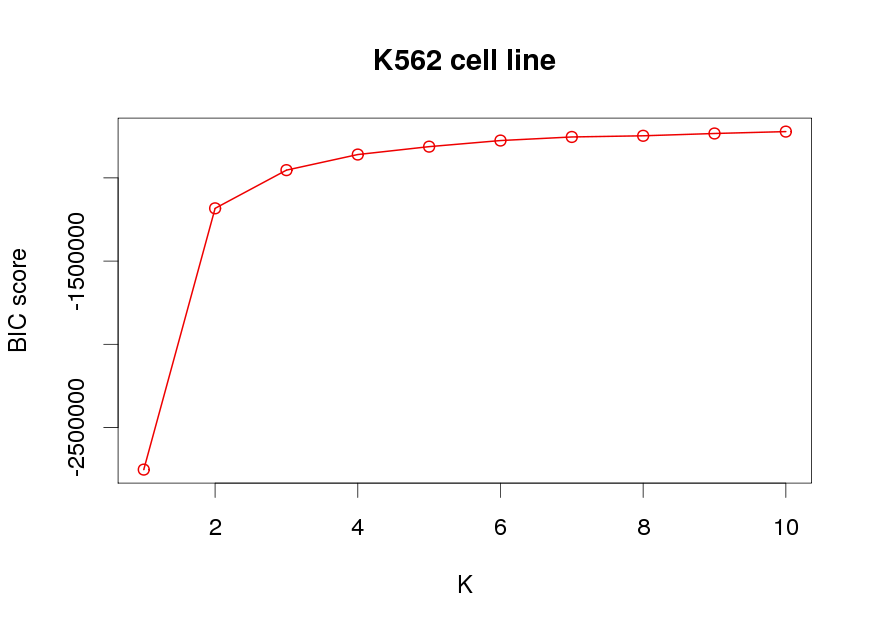
\includegraphics[width=0.48\textwidth]{images/modSelectionK562}
        }
        \subfigure[]{
           \label{model:second}
           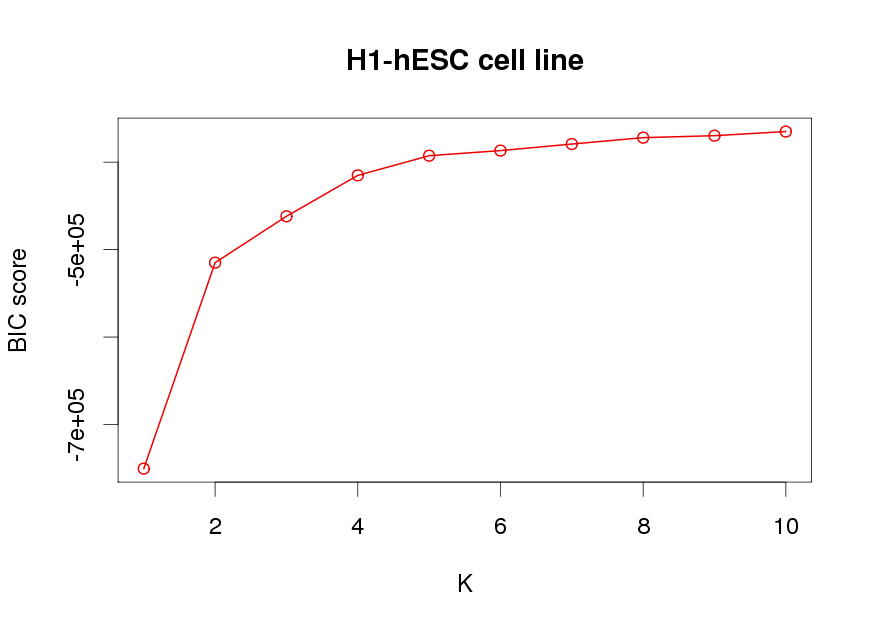
\includegraphics[width=0.48\textwidth]{images/modSelectionH1}
        }
    \end{center}
    \caption{\emph{BIC score as the number of clusters K increases for (a) K562 cell line and (b) H1-hESC cell line.}}
   \label{model-BIC-pic}
\end{figure}